% poster-exemplo (versão minimalista)
% http://www.vision.ime.usp.br/~jmena/stuff/poster-exemplo/
%
% Sáb Nov 12 16:20:02 BRST 2011
%
% OBSERVAÇÕES:
%  - Este exemplo de poster foi adaptado (em 08/2010) considerando os modelos:
%    (a) https://teamwork.jacobs-university.de:8443/confluence/display/CoPandBiG/LaTeX+Poster
%    (b) http://www.nathanieljohnston.com/2009/08/latex-poster-template/
%
%  - Veja as dimensões dos posters em: 
%    http://www.theinternetprinter.com.au/info/A4_A3_A2_A1_A0_Size_Explained.aspx
%

\documentclass[final]{beamer} 
\usepackage[size=b1, orientation=portrait]{beamerposter} % font scale factor=1.0

\usepackage[brazilian]{babel}
\usepackage[utf8]{inputenc}
\usepackage{lmodern}
\usepackage{clrscode3e}                 % para formatar algoritmos como o CLRS
\usepackage{pgfplots}

% cores utilizadas para os algoritmos
\usepackage{framed}
\definecolor{treinamento}{rgb}{0.76471,0.81176,0.91373}  % c3cfe9 -> 195,207,233 -> 0.76471   0.81176   0.91373
\definecolor{reconstrucao}{rgb}{0.83529,0.80784,0.89804} % d5cee5 -> 213,206,229 -> 0.83529   0.80784   0.89804
\definecolor{n_red}{HTML}{D7191C}
\definecolor{n_orange}{HTML}{FD9B61}
\definecolor{n_green}{HTML}{3F745A}
\definecolor{n_green_bg}{HTML}{AAE6C9}
\definecolor{n_blue}{HTML}{2B83BA}
\definecolor{n_violet}{HTML}{AC146D}
\definecolor{n_yellow}{HTML}{D2D221}
\definecolor{RawSienna}{cmyk}{0,0.72,1,0.45}
\definecolor{olive}{rgb}{0.3, 0.4, .1}

\newcommand{\colorize}[2]{\textbf{\textcolor{#1}{#2}}}

\graphicspath{{./figures/}}  
\urlstyle{same}

%\pgfplotsset{every axis/.append style={
%	font=\large,
%	line width=1pt,
%	tick style={line width=1pt}}}


%==The poster style============================================================
\usetheme{poster-exemplo}            % our poster style
%--set colors for blocks (without frame)---------------------------------------
  \setbeamercolor{block title}{fg=ngreen,bg=white}
  \setbeamercolor{block body}{fg=black,bg=white}
%--set colors for alerted blocks (with frame)----------------------------------
%--textcolor = fg, backgroundcolor = bg, dblue is the jacobs blue
  \setbeamercolor{block alerted title}{fg=white,bg=dblue!70}%frame color
  \setbeamercolor{block alerted body}{fg=black,bg=dblue!10}%body color
%
%==Titel, date and authors of the poster=======================================
\title{Um Algoritmo de Escalonamento para Redução do Consumo de Energia em
Computação em Nuvem}
\author{\hskip 10.9cm Pedro Paulo Vezzá Campos \hskip 1cm \url{pedrovc@ime.usp.br} \and \\  Orientador: Prof. Dr. Daniel Macêdo Batista \hskip 1cm \url{batista@ime.usp.br}}
\institute{Departamento de Ciência da Computação --- Instituto de Matemática e 
Estatística --- Universidade de São Paulo}


%==============================================================================
%==the poster content==========================================================
%==============================================================================
\begin{document}
%--the poster is one beamer frame, so we have to start with:
\begin{frame}[t]
%--to seperate the poster in columns we can use the columns environment
\begin{columns}[t] % the [t] options aligns the columns content at the top
%--the left column-------------------------------------------------------------
%\begin{column}{0.28\paperwidth}% the right size for a 3-column layout
\begin{column}{0.35\paperwidth}% the right size for a 3-column layout

	\begin{alertblock}{Introdução}
		TI é responsável por aproximadamente
		2\% das emissões anuais de $CO_2$, próximo do nível gerado pela aviação
		\cite{gartner:co2}. Ao mesmo tempo, a \colorize{RawSienna}{Lei de Moore}, que profetiza que o poder computacional de dispositivos
		dobra a cada 18 meses, está chegando ao fim da sua vida \cite{patterson:computer_organization}.
		Processadores modernos atingiram uma barreira de potência mas no entanto
		não eram eficientes no \colorize{olive}{consumo energético} \cite{barroso:case_energy_proportional}. Assim, novas
		tendências surgiram na indústria: processadores mais simples, mais 
		paralelos e mais eficientes.

		\vskip2ex
		
		\colorize{n_red}{Computação em nuvem} surgiu como uma consequência quase natural destas
		tendências. Ao consolidar poder de processamento, transferência de dados
		e armazenamento é possível reduzir custos e desperdícios. Algumas
		estratégias possíveis: \colorize{n_green}{consolidação} de máquinas virtuais,
		dimensionamento de tensão e frequência (\colorize{n_blue}{DVFS}) e
		\colorize{n_violet}{algoritmos energeticamente eficientes}.
		
		\vskip2ex
		
		Aplicações de processamento paralelo podem ser modeladas como
		\colorize{RawSienna}{digrafos acíclicos} (DAGs). O problema de decidir
		qual o melhor \colorize{n_blue}{escalonamento} de uma tarefa (vértice do DAG) em uma máquina
		de forma a otimizar o uso de algum recurso é um problema \colorize{n_red}{NP-difícil}.
		Assim, heurísticas são necessárias para encontrar soluções aproximadas.
	\end{alertblock}
		
		\vskip2ex
		
	\begin{alertblock}{Resultados}
		Este TCC apresenta
		um \colorize{n_red}{novo algoritmo} de escalonamento de fluxos de
		trabalho em computação em nuvem voltado para a eficiência energética.
		O desempenho foi comparado com o trabalho ``\emph{Energy-aware
		simulation with DVFS}'' \cite{guerout:energy_aware_simulation} 
		e com um algoritmo de escalonamento clássico mas sem um foco na
		eficiência energética. Os estudos contaram com a
		contribuição da aluna de mestrado \colorize{RawSienna}{Elaine Naomi Watanabe}
		(\url{elainew@ime.usp.br}).

		\vskip2ex

		Como resultados secundários, foram feitas \colorize{olive}{contribuições}
		a projetos de \colorize{n_violet}{software livre} na forma de divulgação de código fonte,
		incrementos e notificações de falhas nos simuladores de computação em
		nuvem utilizados pelo autor.
	\end{alertblock}

%	\begin{block}{Modelagem}
%	\begin{columns}[totalwidth=0.34\paperwidth]
%		\begin{column}{0.17\paperwidth}
%			Podemos modelar aplicações de processamento paralelo a serem computadas como um
%			\colorize{RawSienna}{digrafo acíclico} (DAG). Um exemplo, é a aplicação Montage da figura
%			ao lado, que produz mosaicos astronômicos. Dúvida: como associar uma
%			tarefa a uma máquina de forma a diminuir o tempo de processamento ou
%			energia consumida? O problema de encontrar um
%			\colorize{n_blue}{escalonamento} ótimo é \colorize{n_red}{NP-difícil}!
%		\end{column}
%		\begin{column}{0.17\paperwidth}
%			\begin{center}
%				\includegraphics[width=0.9\columnwidth]{Montage_PP.png}
%			\end{center}
%		\end{column}
%	\end{columns}
%	\end{block}
\end{column}

% ---------------------------------------------------------------------------- %
\begin{column}{0.60\paperwidth} 
	\begin{block}{Escalonamento de fluxos de trabalho com computação em nuvem}
		\begin{columns}[totalwidth=0.60\paperwidth]
		\begin{column}{0.33\paperwidth}
			O \emph{Heterogeneous Earliest Finish Time} (\colorize{black}{HEFT})
			\cite{topcoglu:heft} é uma boa heurística para o
			problema de escalonamento. Ele recebe como parâmetros um DAG a ser
			escalonado, um conjunto possivelmente heterogêneo de máquinas que
			realizarão o processamento, os tempos de processamento de cada tarefa
			em cada máquina e o tempo de transmissão entre duas tarefas. Ele
			é dividido em duas fases: \colorize{olive}{priorização} e 
			\colorize{n_violet}{seleção}. 
	
			\vskip2ex

			\begin{block}{Priorização}
			\colorize{n_red}{Qual tarefa escalonar primeiro?} 
			A fórmula abaixo é o critério de priorização do HEFT. Além de gerar
			uma \colorize{n_violet}{ordem topológica}, dá prioridade a tarefas
			mais críticas do DAG.

%			O algoritmo deve obedecer às precedências impostas pelo DAG e ao
%			mesmo tentar dar prioridade a tarefas no \colorize{RawSienna}{caminho
%			crítico}.
			
			$$ \label{eq:rank} rank_u(n_i) = \overline{w_i} + \max_{n_j \in succ(n_i)} (\overline{c_{i,j}} + rank_u(n_j)) $$
				
			\end{block}

			\begin{block}{Seleção}
				\colorize{n_red}{Em qual máquina escalonar uma tarefa?} O HEFT
				tenta minimizar o \colorize{n_blue}{tempo mais cedo de conclusão}
				de cada tarefa na esperança que isso minimize a conclusão do
				fluxo de trabalho como um todo.
			\end{block}
		
%			O \colorize{black}{HEFT} é dividido em dois momentos: No primeiro, define quais tarefas
%			escalonar primeiro. O segundo aloca cada tarefa em ordem de prioridade
%			de maneira a minimizar o tempo mais cedo de conclusão dela.
		

			\definecolor{shadecolor}{named}{treinamento}
			\begin{shaded}
			\begin{codebox}
			\Procname{$\proc{Heterogeneous-Earliest-Finish-Time}()$}
			\li	Defina os custos computacionais das tarefas e os cus-
			\zi tos de de comunicação das arestas com valores médios
		
			\li	Calcule $rank_u$ para todas as tarefas varrendo o grafo
			\zi de ``baixo para cima'',	iniciando pela tarefa final.
		
			\li Ordene as tarefas em uma lista de escalonamento utilizando
			\zi uma ordem não crescente de valores de $rank_u$.
		
			\li 	\While há tarefas não escalonadas na lista
			\li 		\Do
							Selecione a primeira tarefa, $n_i$ da lista de escalonamento.

			\li				\For cada processador $p_k$ no conjunto de processadores
			\li 				\Do
									Calcule o tempo mais cedo de conclusão da tarefa  $n_i$,
			\zi						considerando que ela execute em $p_k$
								\End
			\li				Defina a tarefa $n_i$ para executar no processador $p_j$ que
			\zi					minimiza o tempo mais cedo de conclusão da tarefa $n_i$.
						\End
			\End
			\end{codebox}
			\end{shaded}

		\end{column}
		\begin{column}{0.28\paperwidth}
		\begin{block}{Exemplo}
		Os dados abaixo foram adaptados de \cite{topcoglu:heft}.
			
			\begin{center}
				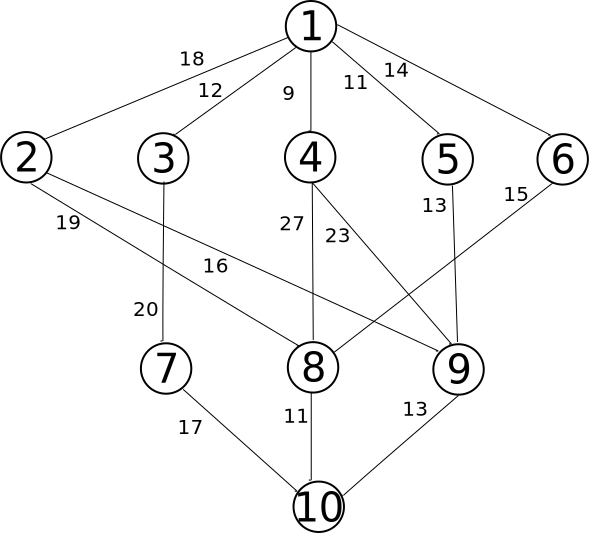
\includegraphics[width=0.68\columnwidth]{dag_heft.pdf}
			\end{center}	

			\begin{table}[ht]
			\small
			\centering
			\begin{tabular}{|c|c|c|c|c|}
			\hline
			\textbf{Tarefa} & \textbf{P1 (s)} & \textbf{P2 (s)} & \textbf{P3 (s)} & $rank_u(n_i)$ \\ \hline
			1               & 14          & 16          & 9           & 108.000       \\
			2               & 13          & 19          & 18          & 77.000        \\
			3               & 11          & 13          & 19          & 80.000        \\
			4               & 13          & 8           & 17          & 80.000        \\
			5               & 12          & 13          & 10          & 69.000        \\
			6               & 13          & 16          & 9           & 63.333        \\
			7               & 7           & 15          & 11          & 42.667        \\
			8               & 5           & 11          & 14          & 35.667        \\
			9               & 18          & 12          & 20          & 44.333        \\
			10              & 21          & 7           & 16          & 14.667        \\ \hline
			\end{tabular}
			\end{table}		

			\begin{center}
				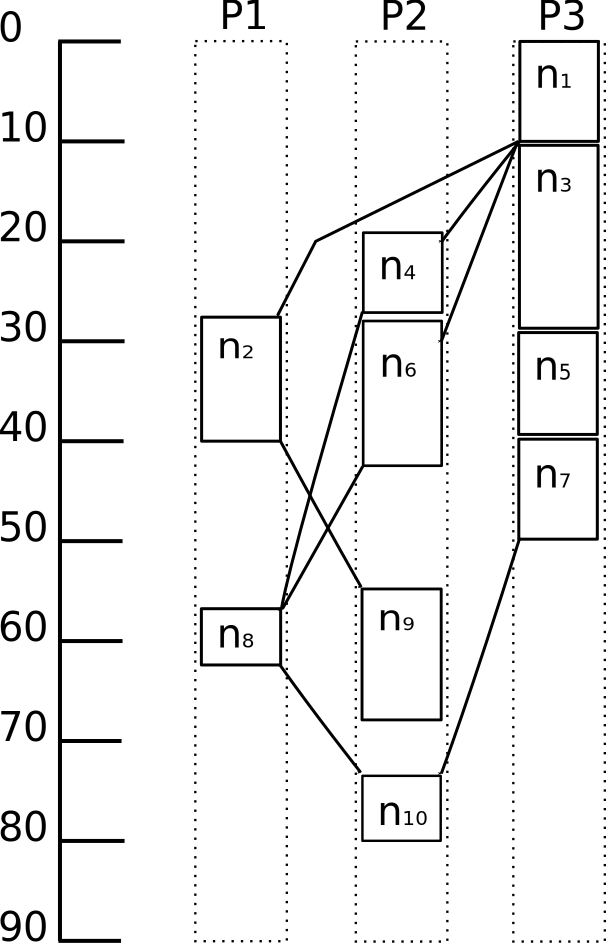
\includegraphics[width=0.42\columnwidth]{escalonamento_heft.pdf}
			\end{center}
		\end{block}	
		\end{column}
		\end{columns}

	\end{block}
	%\vskip2ex

\end{column}
\end{columns}

\vskip2ex

% ---------------------------------------------------------------------------- %

\begin{columns}[t] 
\begin{column}{0.35\paperwidth}

	\begin{block}{Algoritmo Proposto}
	
	\definecolor{shadecolor}{named}{reconstrucao}
	\begin{shaded}
%	\small
	\begin{codebox}
	\Procname{$\proc{EscalonarPowerHEFT}(tarefa, VM)$}
		\li $F \gets \text{filhos diretos da } tarefa \text{ no DAG}$
	    \li Escalone $tarefa$ em $VM$
    	\li Escalone $F$ utilizando o algoritmo \textsc{HEFT}
    	\li \Comment A modelagem energética utilizada está descrita em
	    	\cite{guerout:energy_aware_simulation}
    	\li $energia \gets$ \proc{EstimarEnergiaConsumida()}
  		\li Volte para o escalonamento do começo do laço
    	\li \Return $energia$
	\end{codebox}
	\end{shaded}
	
	
	
	\definecolor{shadecolor}{named}{n_green_bg}
	\begin{shaded}
%	\small
	\begin{codebox}
	\Procname{$\proc{PowerHEFTLookahead}()$}
		\li $V \gets \{VmMaisRápida\}$ \Comment VMs usadas ao escalonar
		\li $O \gets \text{os tipos de VMs que podem ser instanciadas}$
		\li Ordene o conjunto de tarefas segundo o critério $rank_u$
	   
		\li \While há tarefas não escalonadas
			\li \Do $t \gets \text{a tarefa não escalonada de maior } rank_u$
		    \li \Comment Vamos tentar escalonar t em uma VM existente
		    \li \For cada $v$ em $V$:
			    \li \Do	$\proc{EscalonarPowerHEFT}(t, v)$
		    \End
		    
%		    \zi
		    \li \Comment Vamos tentar escalonar t em uma nova VM
		    \li \For cada $o$ em $O$:
			    \li \Do	$V \gets V \cup \{o\}$
			    \li Atualize os valores de $rank_u$
			    \li $t \gets \text{a tarefa não escalonada de maior } rank_u$
			    \li $\proc{EscalonarPowerHEFT}(t, o)$
		    \End
		    
		    \li Escalone $t$ na VM que minimiza a energia consumida
		    \li Atualize $V$ e $rank_u$ caso necessário
		\End
	\End
	\end{codebox}
	\end{shaded}
	
	\end{block}
	
\end{column}

% ---------------------------------------------------------------------------- %
\begin{column}{0.61\paperwidth} 
\begin{block}{Resultados}


\begin{columns}[t] 
	\begin{column}{0.45\columnwidth}
		\begin{center}
			\includegraphics[width=\columnwidth]{Montage.png}
		\end{center}	

		\vskip4ex

		\begin{center}
			\includegraphics[width=\columnwidth]{Sipht.png}
		\end{center}
	\end{column}

	\begin{column}{0.45\columnwidth}
		\begin{center}
			\includegraphics[width=\columnwidth]{CyberShake.png}
		\end{center}	

		\vskip4ex

		\begin{center}
			\includegraphics[width=\columnwidth]{Inspiral.png}
		\end{center}
	\end{column}
\end{columns}

\vskip2ex


\end{block}

\end{column}
\end{columns}

\begin{block}{Referências}
\begin{columns}[t] 
	\begin{column}{0.35\columnwidth}

			\footnotesize{\begin{thebibliography}{99}
			\bibitem[BH07]{barroso:case_energy_proportional}
			L.A. Barroso e U.~H\"olzle.
			The case for energy-proportional computing.
			{\em Computer}, 40(12):33--37, 2007.

			\bibitem[Gar07]{gartner:co2}
			Gartner.
			{Gartner Estimates ICT Industry Accounts for 2 Percent of Global CO2
			  Emissions}, 2007. \url{http://www.gartner.com/newsroom/id/503867}
			[Online; acessado em 7 de dezembro de 2013].

			\end{thebibliography}}

%		\begin{block}{Agradecimentos}
%			O autor gostaria de agradecer os valiosos comentários fornecidos
%			pelo orientador e por Elaine Watanabe, sem os quais este trabalho
%			não teria chegado a este ponto.
%		\end{block}
		
	\end{column}

	\begin{column}{0.30\columnwidth}

			\footnotesize{\begin{thebibliography}{99}
%			\bibitem[PH12]{patterson:computer_organization}
%			D.A. Patterson e J.L. Hennessy. {\em Computer Organization and Design: The Hardware/software
%			  Interface}. Morgan Kaufmann Series in Computer Graphics. Morgan Kaufmann, 2012.

%			\bibitem[BH07]{barroso:case_energy_proportional}
%			L.A. Barroso e U.~H\"olzle.
%			The case for energy-proportional computing.
%			{\em Computer}, 40(12):33--37, 2007.

			\bibitem[GMDC+13]{guerout:energy_aware_simulation}
			Tom Gu{\'e}rout, Thierry Monteil, Georges Da~Costa, Rodrigo Neves~Calheiros,
			  Rajkumar Buyya e Mihai Alexandru.
			Energy-aware simulation with dvfs.
			{\em Simulation Modelling Practice and Theory}, v.39, i.1, p.76-91, 2013.

%			\bibitem[THW02]{topcoglu:heft}
%			H.~Topcuoglu, S.~Hariri e Min-You Wu.
%			Performance-effective and low-complexity task scheduling for
%			  heterogeneous computing.
%			{\em IEEE Transactions on Parallel and Distributed Systems},
%			  13(3):260--274, 2002.

%			\bibitem[Gar07]{gartner:co2}
%			Gartner.
%			{Gartner Estimates ICT Industry Accounts for 2 Percent of Global CO2
%			  Emissions}, 2007.
%			[Online; acessado em 7 de dezembro de 2013].

			\end{thebibliography}}

	\end{column}

	\begin{column}{0.30\columnwidth}

			\footnotesize{\begin{thebibliography}{99}
%			\bibitem[PH12]{patterson:computer_organization}
%			D.A. Patterson e J.L. Hennessy. {\em Computer Organization and Design: The Hardware/software
%			  Interface}. Morgan Kaufmann Series in Computer Graphics. Morgan Kaufmann, 2012.

%			\bibitem[BH07]{barroso:case_energy_proportional}
%			L.A. Barroso e U.~H\"olzle.
%			The case for energy-proportional computing.
%			{\em Computer}, 40(12):33--37, 2007.

%			\bibitem[GMDC+13]{guerout:energy_aware_simulation}
%			Tom Gu{\'e}rout, Thierry Monteil, Georges Da~Costa, Rodrigo Neves~Calheiros,
%			  Rajkumar Buyya e Mihai Alexandru.
%			Energy-aware simulation with dvfs.
%			{\em Simulation Modelling Practice and Theory}, v.39, i.1, p.76-91, 2013.

			\bibitem[PH12]{patterson:computer_organization}
			D.A. Patterson e J.L. Hennessy. {\em Computer Organization and Design: The Hardware/software
			  Interface}. Morgan Kaufmann Series in Computer Graphics. Morgan Kaufmann, 2012.

			\bibitem[THW02]{topcoglu:heft}
			H.~Topcuoglu, S.~Hariri e Min-You Wu.
			Performance-effective and low-complexity task scheduling for
			  heterogeneous computing.
			{\em IEEE Transactions on Parallel and Distributed Systems},
			  13(3):260--274, 2002.

			\end{thebibliography}}
	
	\end{column}
\end{columns}
\end{block}

% ---------------------------------------------------------------------------- %
\end{frame}
\end{document}
